\documentclass{article}
\usepackage{fullpage}
\usepackage{indentfirst}
\usepackage{amsmath}
\usepackage{amsfonts}
\usepackage{array}
\usepackage{tipa}
\usepackage{tikz}
\usepackage{tikz-qtree}
\usetikzlibrary{matrix, arrows, automata}
\usepackage{gb4e}
\noautomath
\newcommand{\Y}{$\checkmark$}
\newcommand{\N}{\ding{55}}
\newcommand{\R}{$\Rightarrow$}
\newcommand\myeq{\mathrel{\stackrel{\makebox[0pt]{\mbox{\normalfont\tiny def}}}{=}}}
\title{Representations: Yip (1989) vs Bao (1990)}
\author{Chris Oakden}
\begin{document}
\maketitle
The purpose here is to offer explicit model-theoretic characterizations of both Yip's (1989) and Bao's (1990) tonal geometry models, and to perform some transductions to translate between them.
\section{Model-theoretical characterization: relations}
We begin by defining models over both representations, starting with a high tone [H]. Recall the models: \\
\begin{center}
Bao 1990
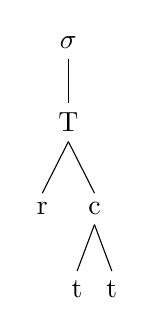
\begin{tikzpicture}[baseline = (current bounding box.north)]
\Tree [.$\sigma$ [.T [.r ] [.c [.t ] [.t ]]]] 
\end{tikzpicture}
\hspace{1cm}
Yip 1989
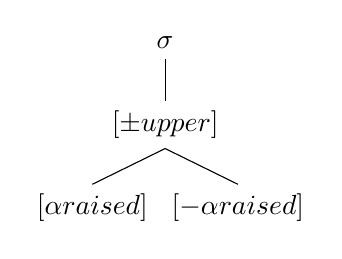
\begin{tikzpicture}[baseline = (current bounding box.north)]
\Tree [.$\sigma$ [.$[\pm upper]$ [.$[\alpha raised]$ ] [.$[-\alpha raised]$ ]]]
\end{tikzpicture} \\ \smallskip{}
\textit{Figure 1: Tonal Geometries in Bao (1990) and Yip (1989)}
\end{center}
In these models, the tonal root node T in Bao's model and the register node ([$\pm$upper]) in Yip's model are equivalent. The terminal tonal nodes are also equivalent, with small `h' and `l' corresponding to the features [+raised] and [-raised] respectively.\par
A high tone in tonal geometry formalism would thus be: \\
\begin{center}
 Bao 1990
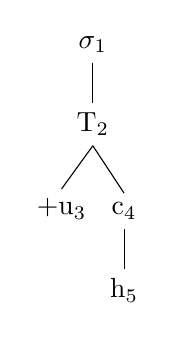
\begin{tikzpicture}[baseline = (current bounding box.north)]
\Tree [.$\sigma_{1}$ [.T$_{2}$ [.+u$_{3}$ ] [.c$_{4}$ [.h$_{5}$ ]]]] 
\end{tikzpicture}
\hspace{1cm}
Yip 1989
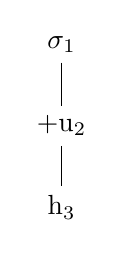
\begin{tikzpicture}[baseline = (current bounding box.north)]
\Tree [.$\sigma_{1}$ [.+u$_{2}$ [.h$_{3}$ ]]]
\end{tikzpicture} \\ \smallskip{}
\textit{Figure 2: H Tone Representation in Two Models}
\end{center}
We can create models for each. They are already numbered for us as individual elements in the model. We define the Yip model on an alphabet $\Sigma = \{\sigma, +u, h\}$. 
\begin{equation} \label{YHmodel1}
\begin{split}
\mathcal{M}^{Y}_{H} = \langle \mathcal{D}; &P_{\sigma}, P_{+u}, P_{h}, R_{\delta} \rangle \\
\mathcal{D} &= \{1, 2, 3\} \\
P_{\sigma} &= \{1\} \\
P_{+u} &= \{2\} \\
P_{h} &= \{3\} \\
R_{\delta} &= \{(1,2), (2,3)\} 
\end{split}
\end{equation}
The model $\mathcal{M}^{Y}_{H}$ defines unary relations for each of the syllable, the register (root) node, and the terminal tonal node, as well as a binary relation $\delta$ for immediate dominance. The relation between tones and TBUs is commonly understood to be association, which we have not yet introduced into the model. Under the assumption that dominance is \emph{not} reflexive, perhaps it is better to introduce a binary association relation. But which elements should be in which relation? A reasonable approach in line with conventional attitudes defines association between the tonal root node (in this case [$\pm$upper]) and the TBU (in this case the syllable), with the dominance relation holding only within the internal structure of the tones themselves. Let us append the model in (\ref{YHmodel1}) to reflect this assumption.
 \begin{equation}
\begin{split}
\mathcal{M}^{Y}_{H} = \langle \mathcal{D}; &P_{\sigma}, P_{+u}, P_{h}, R_{\circ}, R_{\delta} \rangle \\
\mathcal{D} &= \{1, 2, 3\} \\
P_{\sigma} &= \{1\} \\
P_{+u} &= \{2\} \\
P_{h} &= \{3\} \\
R_{\circ} &= \{(1,2)\}  \\
R_{\delta} &= \{(2,3)\} 
\end{split}
\end{equation}
The alphabet for the same structure is larger in Bao's model given the presence of the tonal root node T and the contour node c in the representation: $\Sigma = \{\sigma, T, +u, c, h\}$. Two additional unary predicates are required to construct the model $\mathcal{M}^{B}_{H}$.
\begin{equation}
\begin{split}
\mathcal{M}^{B}_{H} = \langle \mathcal{D}; P_{\sigma}, P_{T}, &P_{+u}, P_{c}, P_{h}, R_{\circ}, R_{\delta} \rangle \\
\mathcal{D} &= \{1, 2, 3, 4, 5\} \\
P_{\sigma} &= \{1\} \\
P_{T} &= \{2\} \\
P_{+u} &= \{3\} \\
P_{c} &= \{4\} \\
P_{h} &= \{5\} \\
R_{\circ} &= \{(1,2)\} \\
R_{\delta} &= \{(2,3), (2,4), (4,5)\}
\end{split}
\end{equation}
With these two models, we can now attempt to perform transductions from one representation to another.
\section{Transduction: relations}
Let $\tau^1$ be a transduction mapping $\mathcal{M}^{Y}_{H}$ to $\mathcal{M}^{B}_{H}$. Let $\tau^2$ be a transduction mapping $\mathcal{M}^{B}_{H}$ to $\mathcal{M}^{Y}_{H}$. My understanding of transduction is a map from one model to another, defined by a set of logical formulas for each relation in the resultant formula, interpreted with respect to the input structure of the original model. I will first attempt to define the transduction $\tau^2$. The definitions of the formulas are presented below:
\begin{equation}
\begin{split}
&\tau^2 \\
P^{\tau^2}_{\sigma}(x) &\myeq P_{\sigma}(x) \\
P^{\tau^2}_{+u}(x) &\myeq P_{+u}(x) \\
P^{\tau^2}_{h}(x) &\myeq P_{h}(x) \\
R^{\tau^2}_{\circ}(x,y) &\myeq P_{\sigma}(x)\,\wedge\,P_{+u}(y) \\
R^{\tau^2}_{\delta}(x,y) &\myeq P_{+u}(x)\,\wedge\,P_{h}(y) 
\end{split}
\end{equation}
The first three formulas are straight-forward; unary relations on syllables, +u register and terminal tonal node `h' are defined in terms of the unary relations from the Yip model $\mathcal{M}^{Y}_{H}$. These relations are also sufficient to describe the association and dominance relations. In fact, since the internal structure of the models is different ($\delta$(+u,h) in $\mathcal{M}^{Y}_{H}$ but not $\mathcal{M}^{B}_{H}$; $\circ$($\sigma$,T) in $\mathcal{M}^{B}_{H}$ but $\circ$($\sigma$,+u) in $\mathcal{M}^{Y}_{H}$), we should avoid using the binary relations from the signature of one model to define the other. Note that this transduction is QF. \par
The transduction $\tau^1$ is not obvious; the tonal root node `T' and the contour node `c' are not defined in the input signature of $\mathcal{M}^{Y}_{H}$, nor are they in the alphabet. One way to derive these is to reference the binary relations of association and immediate dominance. Given the equivalency of the T node (Bao) and the register node (Yip), we can define the former from the latter by way of the input association relation; in other words, the T node is ``that thing which associates to the syllable in the `input' model''. Somewhat ironically, the register node's position in Yip's model (as that which dominates the tonal terminal node) is also equivalent to the contour `c' node in $\mathcal{M}^{B}_{H}$, and can be derived using the input relation $\delta$. I have only been able to define these using existential quantification, so this transduction is not QF (yet). Two symbols $\lambda^{T}$ and $\lambda^{c}$ as placeholders for longer logical expressions are introduced to help parse the definition of the relation $R^{\tau^1}_{\delta}$.
\begin{equation} 
\begin{split}
&\tau^1 \\
P^{\tau^1}_{\sigma}(x) &\myeq P_{\sigma}(x) \\
P^{\tau^1}_{+u}(x) &\myeq P_{+u}(x) \\
P^{\tau^1}_{h}(x) &\myeq P_{h}(x) \\
P^{\tau^1}_{T}(x) &\myeq \exists y[P_{\sigma}(y)\,\wedge\,R_{\circ}(x,y)] \equiv \lambda^{T} \\
P^{\tau^1}_{c}(x) &\myeq \exists z[P_{h}(z)\,\wedge\,R_{\delta}(x,z)] \equiv \lambda^{c} \\
R^{\tau^1}_{\circ}(x,y) &\myeq P_{\sigma}(x)\,\wedge\,\exists z[P_{\sigma}(z)\,\wedge\,R_{\circ}(x,z)] \\
R^{\tau^1}_{\delta}(x,y) &\myeq \Big(\exists z[P_{\sigma}(z)\,\wedge\,R_{\circ}(z,x)]\,\wedge\,P_{+u}(y)\Big)\,\lor \\
&\ \ \ \ \Big(\exists(z,v)[P_{\sigma}(z)\,\wedge\,R_{\circ}(z,x)\,\wedge\,P_{h}(v)\,\wedge\,R_{\delta}(y,v)\Big)\,\lor \\
&\ \ \ \ \Big(\exists z[P_{h}(z)\,\wedge\,R_{\delta}(x,z)]\,\wedge\,P_{h}(y)\Big) \\
&\ \ \ \ \equiv \big(\lambda^{T}(x)\wedge P_{+u}(y)\big)\lor\big(\lambda^{T}(x)\wedge\lambda^{c}(y)\big)\lor\big(\lambda^{c}(x)\wedge P_{h}(y)\big)
\end{split}
\end{equation}
The first three definitions proceed as they did in $\tau^2$. As described above, the `input' association and dominance relations are employed to define `T' and `c' nodes, respectively. The `T' node is identified as the co-associate with the syllable in the `input' signature, while the `c' node is distinguished as the dominator of the terminal `h' node. With these definitions, the `output' association relation between syllable and root node is straightforward. The direct dominance relation is also definable; its three disjuncts represent $\delta$(T, +u), $\delta$(T,c), and $\delta$(c,h).
\section{Interim summary}
Comparing the two tonal geometries, there is an intuition that Bao's model is more complex than Yip's model. This intuition was, in some senses, borne out by performing transductions on them. Yip's model is QF-interpretable from Bao's model, but Bao's model is (as yet) FO-interpretable from Yip's model. \par
In the next sections, we modify our models and conceive of dominance and association as \emph{functions} to determine whether or not it is possible to construct transductions between the models both of which are QF.
\section{Model-theoretic characterization: functions}
The transduction from Yip's model to Bao's model required the use of existential quantification, and was thus of a greater logical complexity than the inverse transduction. These models used only relations; will we achieve a different result by representing binary relations as unary functions? More specifically, can we posit transductions $\tau1$ and $\tau2$ that are both QF (such that the representations are QF-interpretable)? This section will replace the two binary relations $R_{\circ}$ and $R_{\delta}$ with functions $\alpha(x)$ for association and $\delta(x)$ for immediate dominance with this result in mind. \par
Below is a model $\mathcal{M}^{Y'}_{H}$ for a H tone using Yip's representation. The alphabet is identical to that in the relation-only model.
 \begin{equation}
\begin{split}
\mathcal{M}^{Y'}_{H} = \langle \mathcal{D}; &P_{\sigma}, P_{+u}, P_{h}, \alpha(x), \delta(x) \rangle \\
\mathcal{D} &= \{1, 2, 3\} \\
P_{\sigma} &= \{1\} \\
P_{+u} &= \{2\} \\
P_{h} &= \{3\} \\
\alpha(x) &= \begin{cases} 2 & x=1 \\
				     1 & x=2  \end{cases} \\
\delta(x) &= \begin{cases} 3 & x = 2 \end{cases} 
\end{split}
\end{equation}
Two observations are worth noting here. One is that the functions are not total functions. Given the simplicity of this model, it would appear that defining either $\alpha(x)$ or $\delta(x)$ as total would be unproblematic. It will become clear when examining Bao's model that total functions are not desirable. In other words, we don't a total association function on a model in which only a single tonal node associates to a single TBU. At least I think that's the case (I'm still not completely sure about how functions work). The second point is that the association function is reflexive-\emph{esque}. That is to say, when the function is evaluated on element 1 in the domain, it returns 2, and vice versa. The impetus for this characterization is in preserving the flavor of the reflexive binary relation. Under the assumption that association doesn't originate from one element (tone or TBU) and project to the other, this way of the defining the function seems to be the most accurate. Again, I'm not sure. \par
Bao's model follows from the relation-only model in the previous sections. Unary relations are identical, and the functions are like those in the function model for Yip. When defining the dominance function, I noticed that there were two distinct codomain elements for the function domain element [2]. In other words, $\delta(2)=3$ and $\delta(2)=4$. This is a problem. $\delta(x)$ is not a function, which means that understanding immediate dominance in binary (or greater) branching structures as functions does not work when the `dominator' is the domain of the function.
 \begin{equation}
\begin{split}
\mathcal{M}^{B'}_{H} = \langle \mathcal{D}; P_{\sigma}, P_{T}, &P_{+u}, P_{c}, P_{h}, \alpha(x), \delta(x) \rangle \\
\mathcal{D} &= \{1, 2, 3, 4, 5\} \\
P_{\sigma} &= \{1\} \\
P_{T} &= \{2\} \\
P_{+u} &= \{3\} \\
P_{c} &= \{4\} \\
P_{h} &= \{5\} \\
\alpha(x) &= \begin{cases} 2 & x=1 \\
				     1 & x=2  \end{cases} \\
\delta(x) &= \begin{cases} 3 & \textbf{x=2}  \\
				     4 & \textbf{x=2} \ \ \ \leftarrow  \text{Oh, crumbs!} \\
				     5 & x=5  \end{cases} \\
\end{split}
\end{equation}
An alternative to this is to understand the $\delta(x)$ function as something like `is immediately dominated by' instead. This results in a function that is surjective but not injective (but at least \emph{is} a well-formed function by definition). See the modified model below.
 \begin{equation}
\begin{split}
\mathcal{M}^{B''}_{H} = \langle \mathcal{D}; P_{\sigma}, P_{T}, &P_{+u}, P_{c}, P_{h}, \alpha(x), \delta(x) \rangle \\
\mathcal{D} &= \{1, 2, 3, 4, 5\} \\
P_{\sigma} &= \{1\} \\
P_{T} &= \{2\} \\
P_{+u} &= \{3\} \\
P_{c} &= \{4\} \\
P_{h} &= \{5\} \\
\alpha(x) &= \begin{cases} 2 & x=1 \\
				     1 & x=2  \end{cases} \\
\delta(x) &= \begin{cases} 2 & x\in(3,4) \\
				     4 & x=5 \end{cases} \\
\end{split}
\end{equation}
The next section re-casts transductions $\tau^1$ and $\tau^2$ (called $\tau^3$ and $\tau^4$ for clarity) using the relational/functional models. 
\section{Transduction: functions}
The logical formulas for transduction $\tau^4$ are mostly identical to $\tau^2$. The difference between the two lies in the definition of association and dominance. In $\tau^2$, association was defined in terms of two unary predicates which were joined in a conjunction to denote the $x$ and $y$ members of the binary relation. We define association also in terms of unary predicates and not the input association function (recall that the association relations are different between the two models), but unite them by means of disjunction. This should reflect the so-called reflexivity of the function. \textcolor{red}{(Wait... is it ok to define a function in terms of unary predicates? Is it the case that both are going to evaluate a truth value? I know that functions don't return truth values, but when defining a function in a transduction, is it something different? This is something that I am unsure about.)}
\begin{equation}
\begin{split}
&\tau^4 \\
P^{\tau^4}_{\sigma}(x) &\myeq P_{\sigma}(x) \\
P^{\tau^4}_{+u}(x) &\myeq P_{+u}(x) \\
P^{\tau^4}_{h}(x) &\myeq P_{h}(x) \\
\alpha^{\tau^4}(x) &\myeq P_{\sigma}(x) \lor P_{+u}(x) \\
\delta^{\tau^4}(x) &\myeq \delta(P_{c}(x))\\ 
\end{split}
\end{equation}
The definition for $\delta^{\tau^4}(x)$ is dissatisfying, but I'm not sure how to change it. What it says essentially is: direct domination is defined as that which was directly dominated by the element corresponding to the node `c' in the input model. In other words, it says that direct domination is defined by the `h' node being dominated. We can identify the dominated, but not the \emph{dominator}. Without an extra free variable, how do we indicate that `h' is dominated by [+u] in the Yip model (whereas it was dominated by `c' in the Bao model)? \textcolor{red}{I'm still unsure how to do this.}\par
In defining the unary predicates in $\tau^3$, we see the value of the functions. Instead of resorting to existential quantification with binary relations, we can define the tonal root node `T' as `the domain element which associates with the syllable' and the contour node `c' as `the domain element which is dominated by the thing that associates with the syllable' \textcolor{red}{(I'm not sure that this is right)}. We can employ the disjunction from $\tau^3$ and the `T' node definition to characterize the output $\alpha^{\tau^4}(x)$ function.
\begin{equation}
\begin{split}
&\tau^3 \\
P^{\tau^3}_{\sigma}(x) &\myeq P_{\sigma}(x) \\
P^{\tau^3}_{+u}(x) &\myeq P_{+u}(x) \\
P^{\tau^3}_{h}(x) &\myeq P_{h}(x) \\
P^{\tau^3}_{T}(x) &\myeq \alpha(P_{\sigma}(x)) \\
P^{\tau^3}_{c}(x) &\myeq \delta(\alpha(P_{\sigma}(x))) \\
\alpha^{\tau^4}(x) &\myeq P_{\sigma}(x) \lor \alpha(P_{\sigma}(x)) \\
\delta^{\tau^4}(x) &\myeq \Big(\delta(P_{+u}(x))\Big)\lor\Big(???\Big)\\ 
\end{split}
\end{equation}
I'm at a loss for how to define the dominance function in this transduction. Using a function $\delta(x)$ to indicate `is dominated by', there are three elements which are dominated in the output model: `h', `+u', and `c'. We could just include those as disjuncts as the `dominated' elements, but it's clear that there is no indication as to what the dominance relationships are.  
\section{A short aside}
I have no idea how to do transductions on functions when they're not identical in both models. In Kristina's work on translating between different syllabic representations, she has dominance as relations. In her Berber paper, she has predecessor and successor functions in her models, but they are preserved in the transductions.\par
How about defining them like they are in the input model \textcolor{red}{(so with a domain and a codomain, but those elements are defined in terms of the input structure?)}? I'll give that a shot here very quickly.
\begin{equation}
\begin{split}
&\tau^4 \\
\alpha^{\tau^4}(x) &= \begin{cases} P_{+u}(x) & x = P_{\sigma}(x) \\
						   P_{\sigma}(x) & x = P_{+u}(x) \end{cases} \\
\delta^{\tau^4}(x) &= \begin{cases} P_{+u} & x = P_{h}(x) \end{cases} 
\end{split}
\end{equation}
\begin{equation}
\begin{split}
&\tau^3 \\
\alpha^{\tau^3}(x) &= \begin{cases} \alpha(P_{\sigma}(x)) & x = P_{\sigma}(x) \\
						   P_{\sigma}(x) & x = \alpha(P_{\sigma}(x)) \end{cases} \\
\delta^{\tau^3}(x) &= \begin{cases} \alpha(P_{\sigma}(x)) & x \in \Big( \delta(\alpha(P_{\sigma}(x))), P_{+u}\Big) \\ 
						   \delta(\alpha(P_{\sigma}(x))) & x = P_{+h} \end{cases}
\end{split}
\end{equation}
\section{New Stuff}
New Definitions of models, specifically making association non-reflexive. 
Yip's model
\begin{equation}
\begin{split}
\mathcal{M}^{Y'}_{H} = \langle \mathcal{D}; &P_{\sigma}, P_{+u}, P_{h}, \alpha(x), \delta(x) \rangle \\
\mathcal{D} &= \{1, 2, 3\} \\
P_{\sigma} &= \{1\} \\
P_{+u} &= \{2\} \\
P_{h} &= \{3\} \\
\alpha(x) &= \begin{cases} 2 & x=1 \end{cases} \\
\delta(x) &= \begin{cases} 3 & x = 2 \end{cases} 
\end{split}
\end{equation}

\begin{equation}
\begin{split}
\mathcal{M}^{B'}_{H} = \langle \mathcal{D}; P_{\sigma}, P_{T}, &P_{+u}, P_{c}, P_{h}, \alpha(x), \delta(x) \rangle \\
\mathcal{D} &= \{1, 2, 3, 4, 5\} \\
P_{\sigma} &= \{1\} \\
P_{T} &= \{2\} \\
P_{+u} &= \{3\} \\
P_{c} &= \{4\} \\
P_{h} &= \{5\} \\
\alpha(x) &= \begin{cases} 2 & x=1 \end{cases} \\
\delta(x) &= \begin{cases} 2 & x\in(3,4) \\
				     4 & x=5 \end{cases} \\
\end{split}
\end{equation}
\end{document}